\chapter{\MakeUppercase{Механическая конструкция}}
\section{Проектирование ног} \label{sec:leg_design}
Основная, и самая сложная с точки зрения механики часть шагающего робота это конечности. Как и корпус, ноги проектировались в виде трёхмерных, твердотельных чертежей. Для уменьшения количества уникальных деталей конструкция всех четырех ног была унифицирована (рисунки \ref{fig:the_same_legs} и \ref{fig:the_same_details}). Таким образом снижена сложность и затратность в производстве деталей. 

\begin{figure}[h]
    \centering
    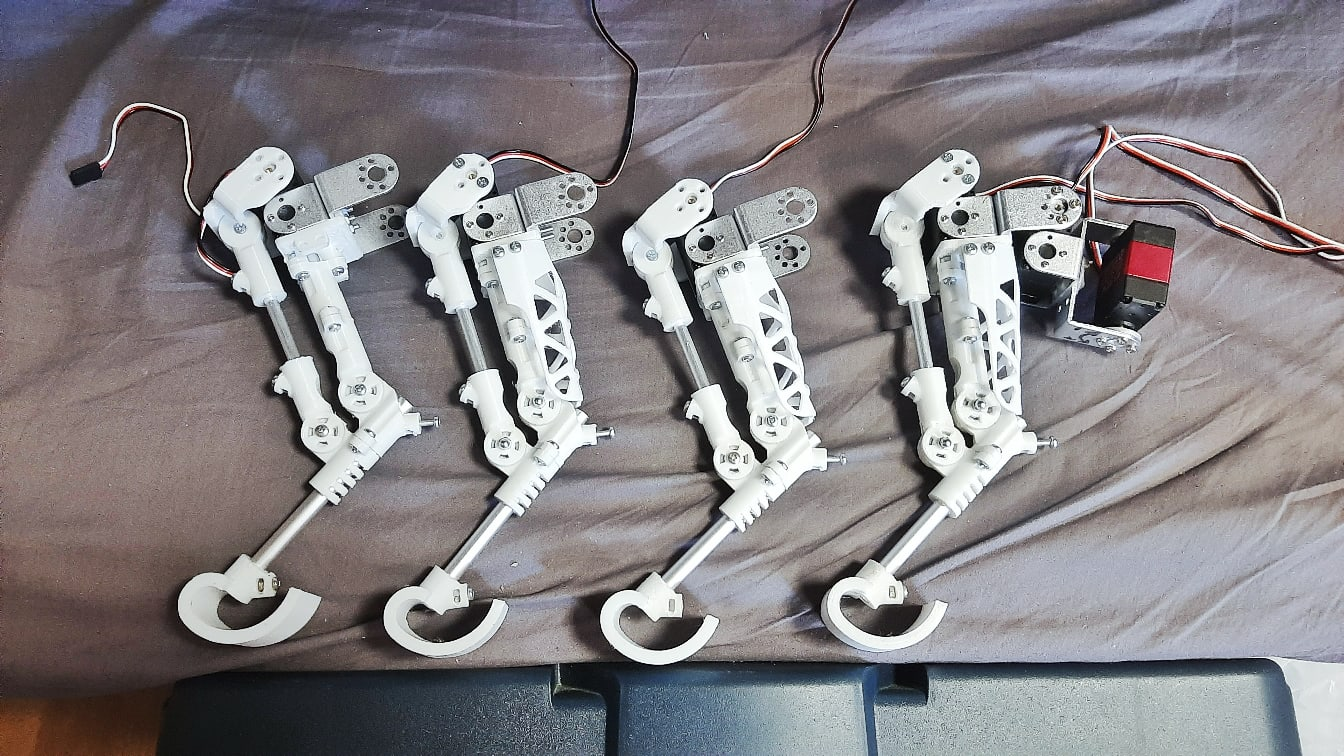
\includegraphics[width=\textwidth]{chapter_mechanics_construction/figure11.jpg}
    \caption{Конструкции всех четырех ног унифицированы}
    \label{fig:the_same_legs}
\end{figure}

Сложные по форме детали изготовлены из пластика на 3D-принтере, в конструкции также присутствуют металлические стержни, стандартные металлические кронштейны, крепежные элементы (винты, гайки).

Перед проектированием были выдвинуты функциональные требования к конечностям. Они должны быть как можно менее габаритными, для сохранности редукторов сервоприводов и для увеличения скорости движения нужно максимально уменьшить момент инерции конечности. Основной способ достижения этой цели -- уменьшение веса всех деталей. Поэтому некоторые крепежи и элементы корпуса, по возможности, были изготовлены из пластика. Были использованы полые цилиндрические аллюминиевые трубки в качестве стержней, обеспечивающих жесткость.

\begin{figure}[h]
    \centering
    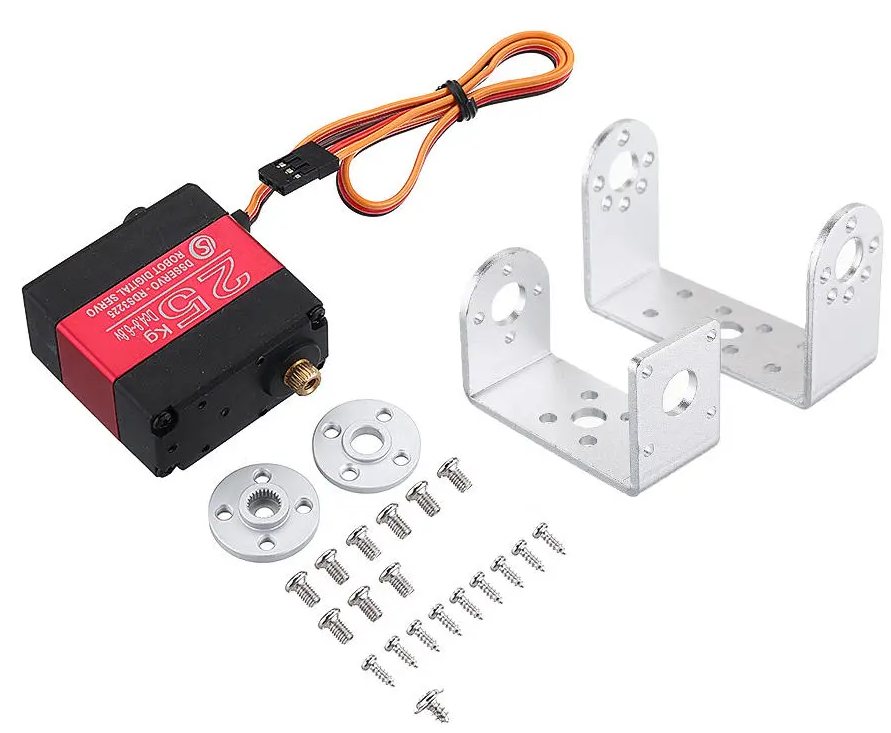
\includegraphics[scale=0.45]{chapter_mechanics_construction/figure6.png}
    \caption{Сервоприводы \textit{DSSERVO RDS3225}, использованные в прототипе робота}
    \label{}
\end{figure}

Есть еще один, не менее эффективный способ снизить момент инерции ног, не уменьшая общего веса конечностей -- концентрация основной массы как можно выше \cite{Seok2012}, ближе к месту крепления ноги к корпусу. Поэтому сервоприводы, как одни из самых тяжелых элементов конструкции, были перенесены как можно ближе к корпусу и как можно дальше от пола. Получившаяся конструкция изображена на рисунке \ref{fig:figg7}.

\begin{figure}[h]
    \centering
    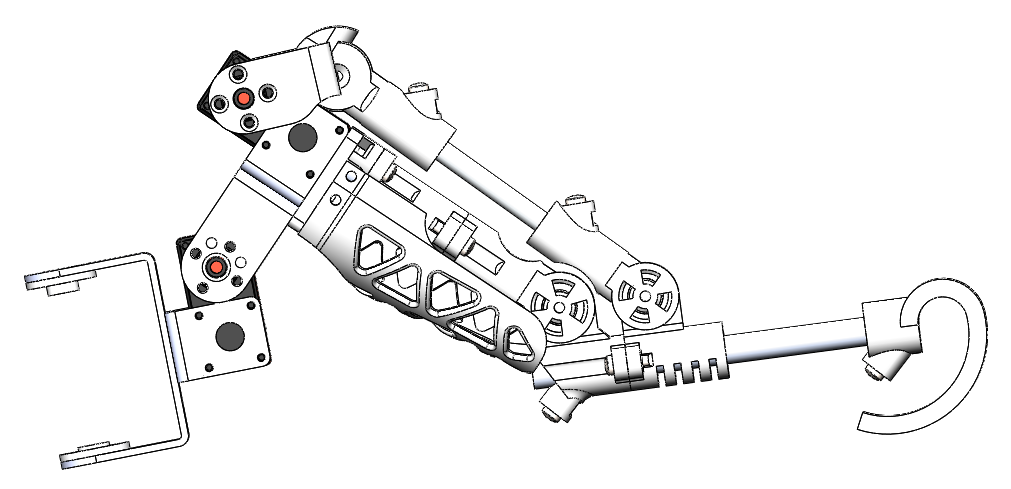
\includegraphics[scale=0.7]{chapter_mechanics_construction/figure7.png}
    \caption{Твердотельный чертеж конечности робота. Можно заметить что двигатели размещены у основания конечности.}
    \label{fig:figg7}
\end{figure}

Двигатель неудобно размещать в узле в силу конструктивных особенностей. В связи с этим в конструкции возник механический четырехзвенник, позволяющий передавать вращение стержневых элементов. Четырехзвенник усложнил кинематическую схему ноги, его расчет рассмотрен далее в пункте \ref{sec:pre_direct_kin}, однако такая конструкция позволила уменьшить габариты конечности и положительно повлияла на её эстетические качества. 

\begin{figure}[h]
    \centering
    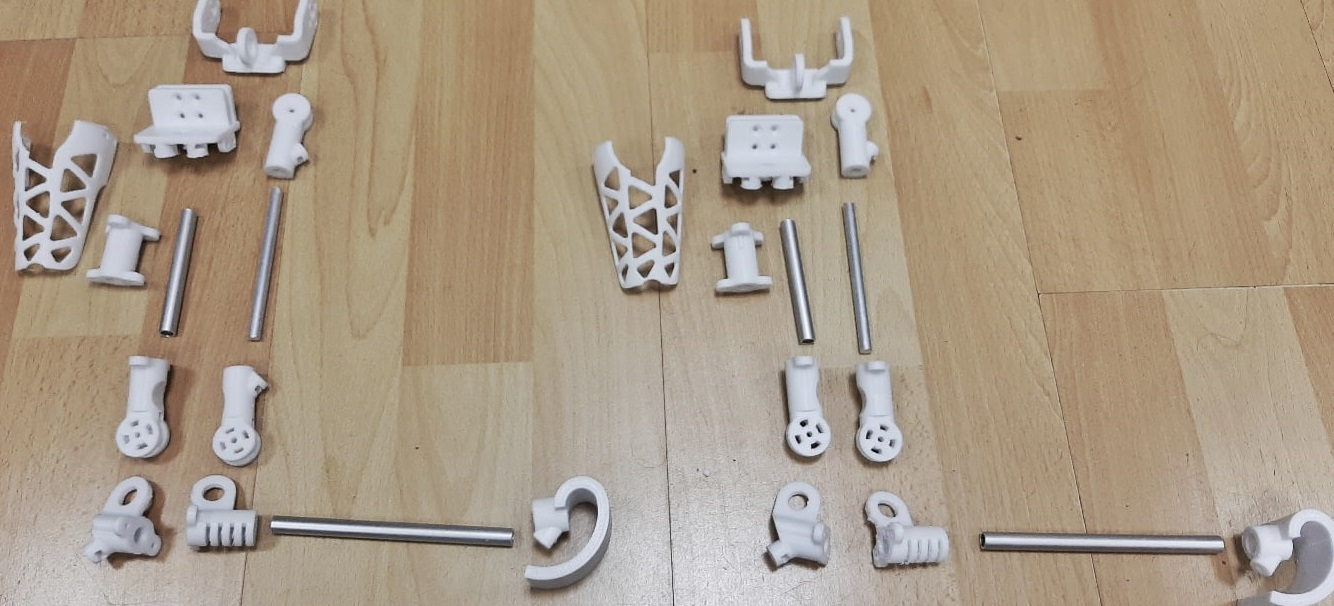
\includegraphics[width=\textwidth]{chapter_mechanics_construction/figure14.jpg}
    \caption{Набор унифицированных деталей для изготовления конечностей.}
    \label{fig:the_same_details}
\end{figure}

\begin{figure}[h]
    \centering
    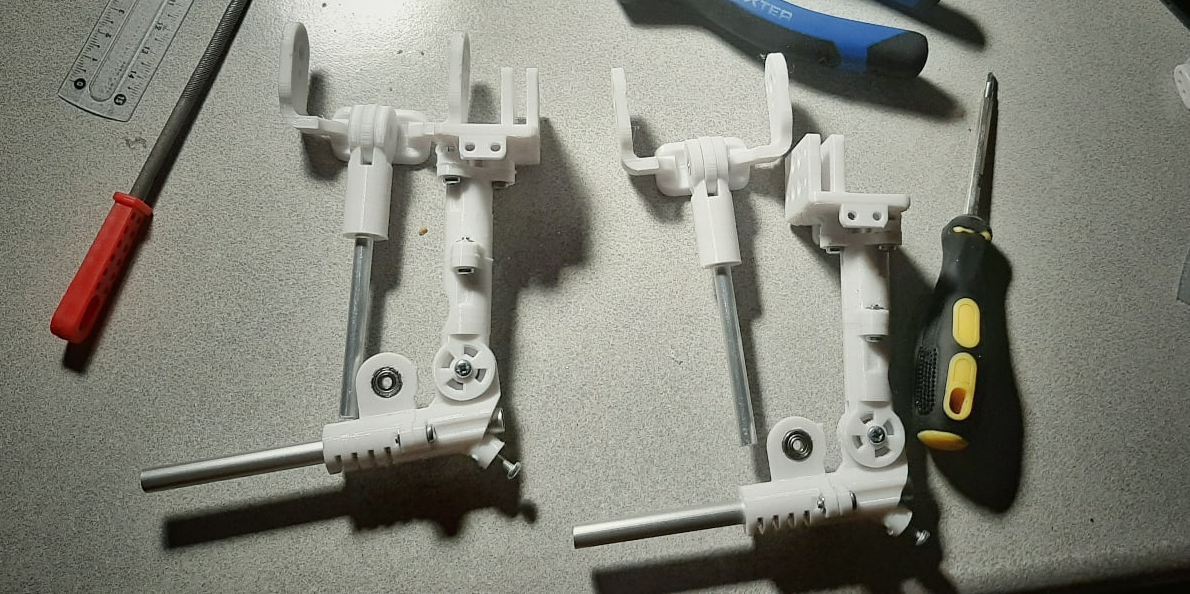
\includegraphics[width=\textwidth]{chapter_mechanics_construction/figure12.png}
    \caption{Процесс сборки конечностей. Используются полые аллюминиевые стержни и пластиковые детали.}
    \label{}
\end{figure}

% ввести термины "стопы" и другие в описании кинематики
\newpage
В конструкции предусмотрена установка датчиков касания на стопы. Конструкция ноги позволит без проблем проложить провода так, чтобы их не было видно.
\begin{figure}[ht]
    \centering
    % левая картинка
    \begin{subfigure}[b]{0.45\textwidth}    
        \centering
        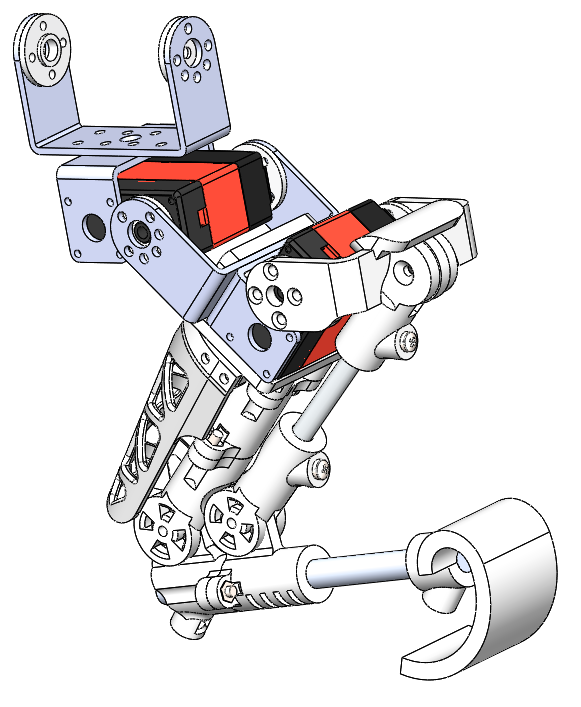
\includegraphics[scale=0.55]{chapter_mechanics_construction/figure15.png}
        \caption{Последнее звено согнуто}
    \end{subfigure}
    % правая картинка  
    \begin{subfigure}[b]{0.45\textwidth}
        \centering
        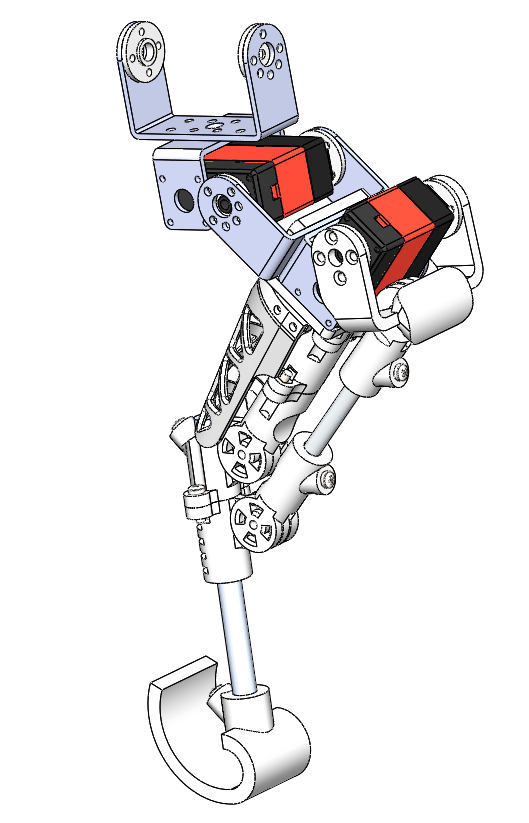
\includegraphics[scale=0.55]{chapter_mechanics_construction/figure16.png}
        \caption{Последнее звено разогнуто}
    \end{subfigure}
     
    \caption{Конечность в двух состояниях}
    \label{}
\end{figure}

Из-за специфики сервоприводов возникают проблемы, которые замедляют процесс сборки и требуют наличия управляющей электроники. В используемых сервоприводах установлены абсолютные датчики угла поворота вала (энкодеры). Такой сервопривод при установке в конструкцию должен быть верно сконфигурирован, или проще говоря, нужно, чтобы вал сервопривода был заранее повернут на известный управляющей программе угол (<<технический>> угол). Эту особеность можно считать минусом, так как в приводах с относительными энкодерами конфигурировать углы поворота при сборке не нужно. Однако во время использования таких приводов нужно проводить калибровку, поворачивая их в нулевое, начальное положение. Перевод в начальное положение подразумевает наличие концевых выключателей в конструкции. Такие приводы не были использованы в силу своей дороговизны и в силу того, что наличие концевых выключателей сильно бы усложнило разработку. Для прототипа это излишне.

\section{Проектирование корпуса}
Требования к корпусу можно разделить на три составляющие: массовые, габаритные и эстетические. Снижать массу нужно для того чтобы разгрузить конечности робота, защитить редукторы электроприводов. Снижению массы способствует максимальный отказ от металлических деталей, а там где это невозможно (в силу требований по жесткости), нужно использовать эффективные сечения профилей, желательно из аллюминия.

В качестве каркаса, к которому крепятся ноги робота, был выбран конструкционный аллюминиевый профиль, из-за его легкости, жесткости и простоты крепления новых деталей к профилю.
\begin{figure}[ht]
    \centering
    % левая картинка
    \begin{subfigure}[b]{0.45\textwidth}    
        \centering
        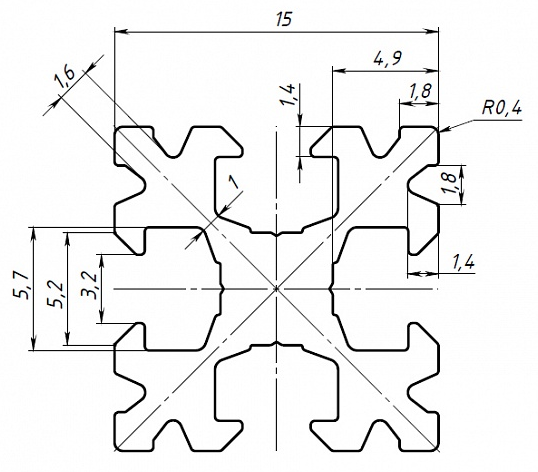
\includegraphics[scale=0.75]{chapter_mechanics_construction/figure8.png}
        \caption{Сечение профиля}
    \end{subfigure}
    % правая картинка  
    \begin{subfigure}[b]{0.45\textwidth}
        \centering
        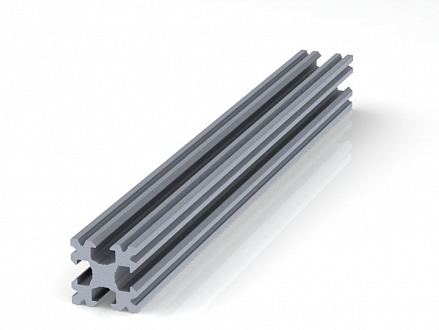
\includegraphics[scale=0.9]{chapter_mechanics_construction/figure9.png}
        \caption{Внешний вид профиля}
    \end{subfigure}
     
    \caption{Конструкционный аллюминиевый профиль}
    \label{}
\end{figure}

Объем корпусу придают тонкие цилиндрические аллюминиевые стержни и пластиковые детали в качестве передней и задней стенок. В узлах между металлическими профилями используются пластиковые крепежи. Такая конструкция позволяет использовать много свободного места внутри корпуса, что упрощает размещение электронных компонентов внутри.

\begin{figure}[h]
    \centering
    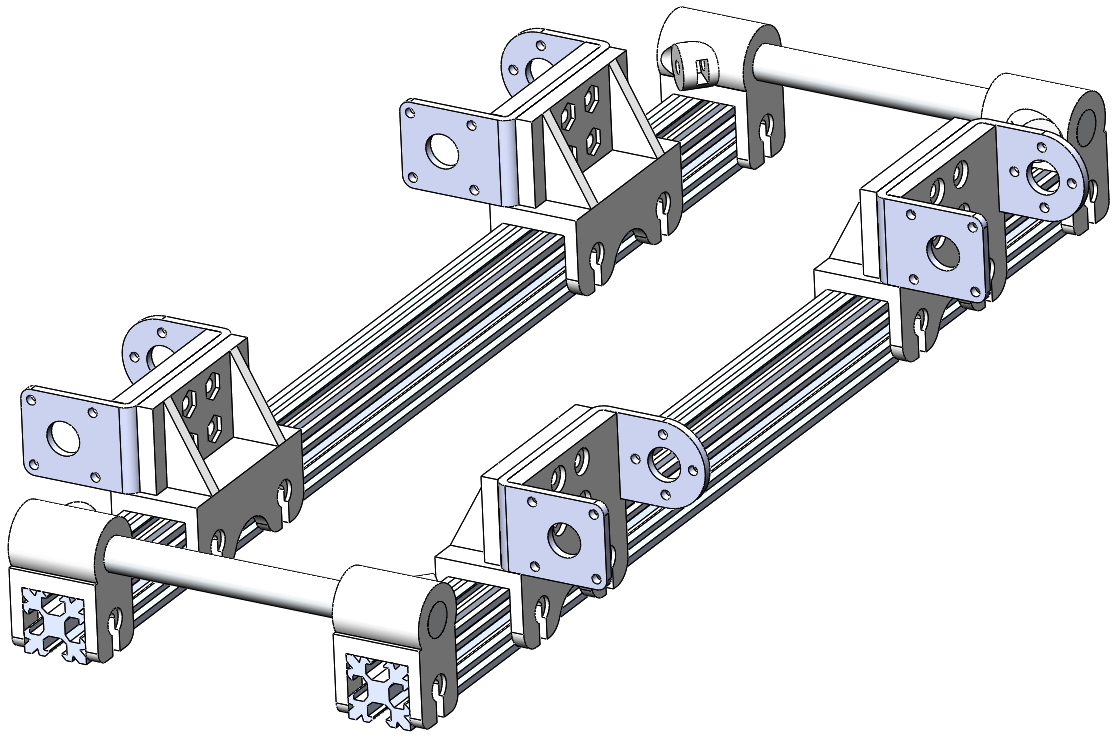
\includegraphics[scale=0.55]{chapter_mechanics_construction/figure10.png}
    \caption{Основной каркас корпуса}
    \label{}
\end{figure}

\newpage
Самой сложной задачей было размещение всех компонентов внутри корпуса, так как нужно обеспечить удобный доступ к ним в любой момент времени для замены или диагностики. Таким образом, повышается общая ремонтопригодность прототипа, а это сильно ускоряет работу с ним.

\begin{figure}[h]
    \centering
    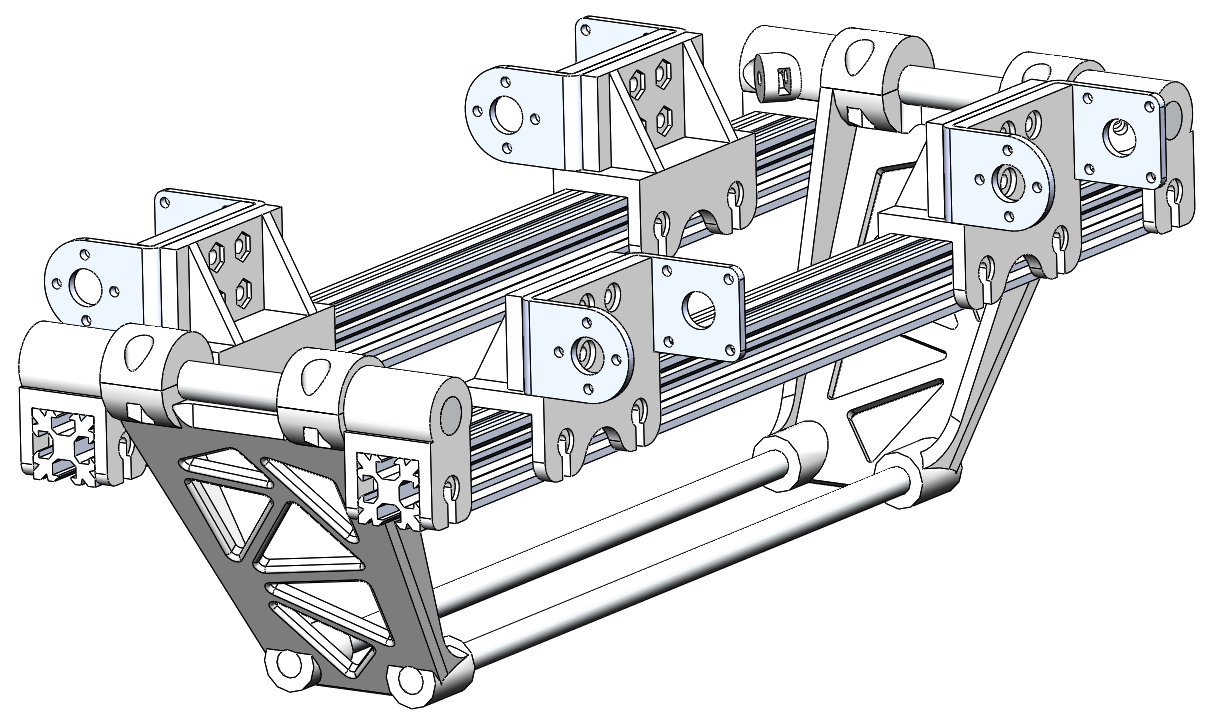
\includegraphics[scale=0.57]{chapter_mechanics_construction/figure13.png}
    \caption{Короб, скрепленный с корпусом}
    \label{}
\end{figure}

Чтобы максимально облегчить работу над монтажем электроники, был разработан электронный блок, целиком вынимающийся из корпусного короба. У такого решения есть как преимущества, так и недостатки. Важно, что в таком состоянии сохраняется <<наглядность>> электронной схемы, легкий доступ воздуха к компонентам, исключающий факт перегрева и последующего выхода из строя по причине того что перегрев не был вовремя замечен.
\begin{figure}[ht]
    \centering
    % левая картинка
    \begin{subfigure}[b]{0.45\textwidth}    
        \centering
        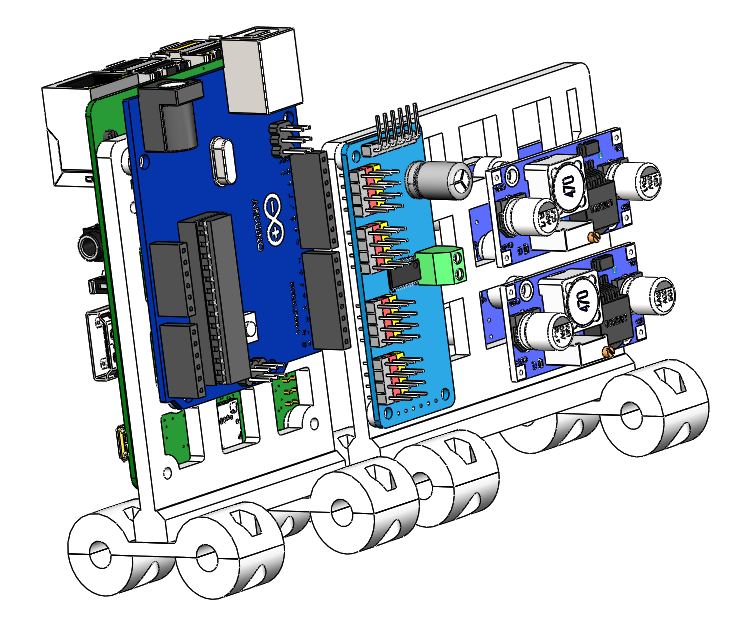
\includegraphics[scale=0.45]{chapter_mechanics_construction/figure17.png}
        \caption{}
    \end{subfigure}
    % правая картинка  
    \begin{subfigure}[b]{0.45\textwidth}
        \centering
        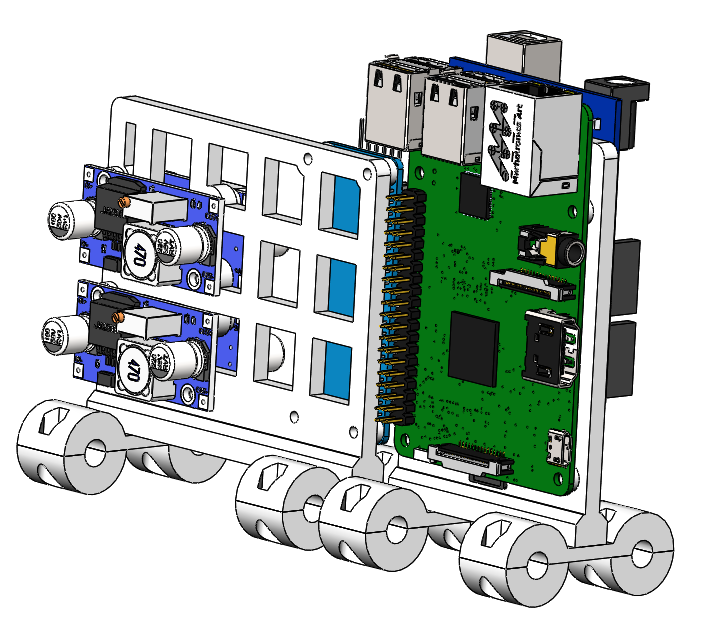
\includegraphics[scale=0.45]{chapter_mechanics_construction/figure18.png}
        \caption{}
    \end{subfigure}
     
    \caption{Электронный блок с разных сторон}
    \label{}
\end{figure}

Такой электронный блок монтируется на стержни нижней части корпуса, что позволяет менять его положение и порядок установки даже после сборки робота. Корпус робота с электронным блоком и аккумулятором представлен на рисунке \ref{fig:full_body}.
\begin{figure}[h]
    \centering
    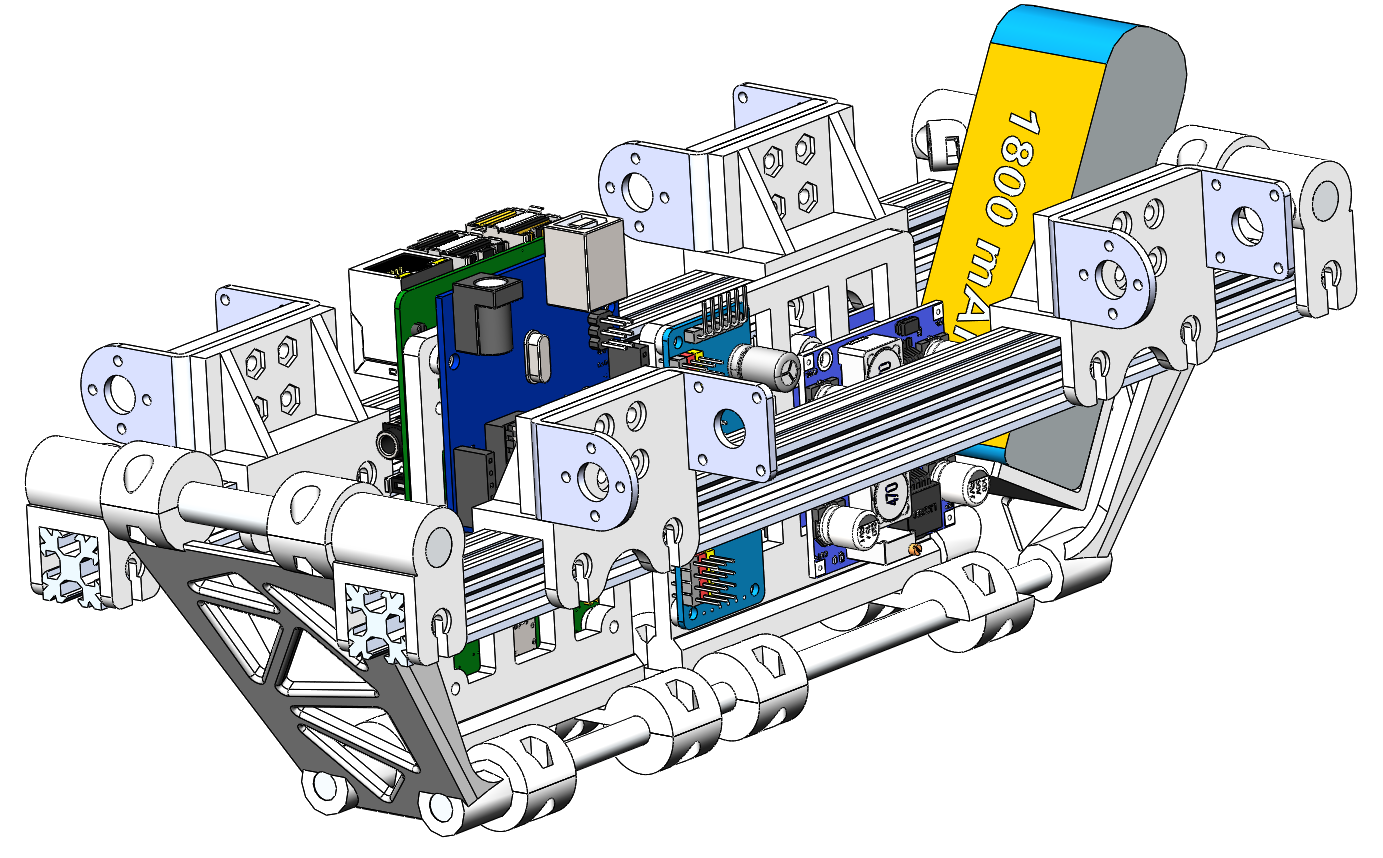
\includegraphics[scale=0.45]{chapter_mechanics_construction/figure19.png}
    \caption{Корпус робота с электронным блоком и аккумулятором}
    \label{fig:full_body}
\end{figure}

\section{Подбор комплектующих}
\subsection{Силовая электроника}
Из силовой электроники в роботе присутствуют:
\begin{itemize}
    \item Сервоприводы
    \item Преобразователи постоянного напряжения.
\end{itemize}

Исходя из ожидаемых моментов и скоростей был выбран заводской сервопривод \textit{DSSERVO RDS3225}.

% Использовать паспортные данные двигателей для расчётов может быть рискованно, нужно измерить их реальный момент вращения. Для измерения крутящих моментов были разработаны стенды, принцип действия которых можно описать схемой на рисунке \ref{fig:stend}:
% \begin{figure}[ht]
%     \centering
%     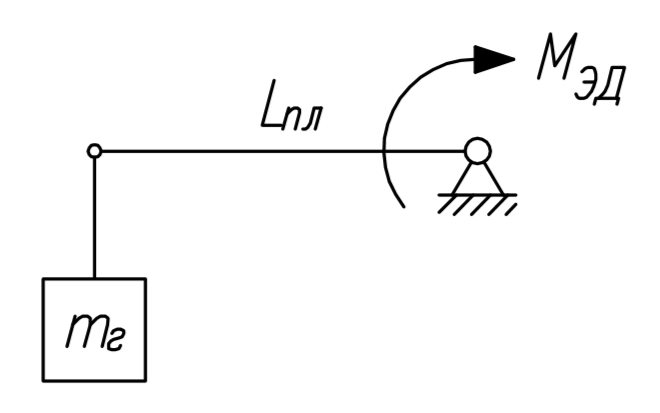
\includegraphics[scale=0.7]{chapter_legged_robots/kin3.png}
%     \caption{Кинематика стенда для измерения крутящего момента}
%     \label{fig:stend}
% \end{figure}

% На рисунке $ m_г $ "--- известная масса груза, которая подвешивалась на разных расстояниях $ L_{пл} $ от вала редуктора. Из приведенных величин можно легко найти экспериментально значение момента $ M_{ЭД} $. 

% Написать о проверке дигателя, но не расписывать стенд. Можно отправить стенд в приложения.

Используются одни из самых компактных и простых в настройке преобразователей напряжения. В основном используются испульсные преобразователи напряжения на базе микросхем \textit{LM-XXXX} и \textit{XL-XXXX}. Они хорошо взаимозаменяемы друг с другом. Для двух пар ног выбраны два преобразователя с максимальным током нагрузки $ 5 \: А $. Для питания логической части используется преобразователь с током нагрузки $ 3 \: А $.
\begin{figure}[ht]
    \centering
    % левая картинка
    \begin{subfigure}[b]{0.45\textwidth}    
        \centering
        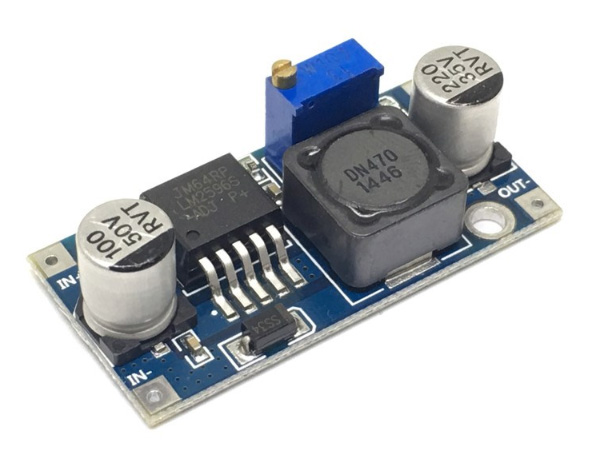
\includegraphics[scale=0.30]{chapter_mechanics_construction/figure4.jpg}
        \caption{Преобразователь на базе \textit{LM2596S}}
    \end{subfigure}
    % правая картинка  
    \begin{subfigure}[b]{0.45\textwidth}
        \centering
        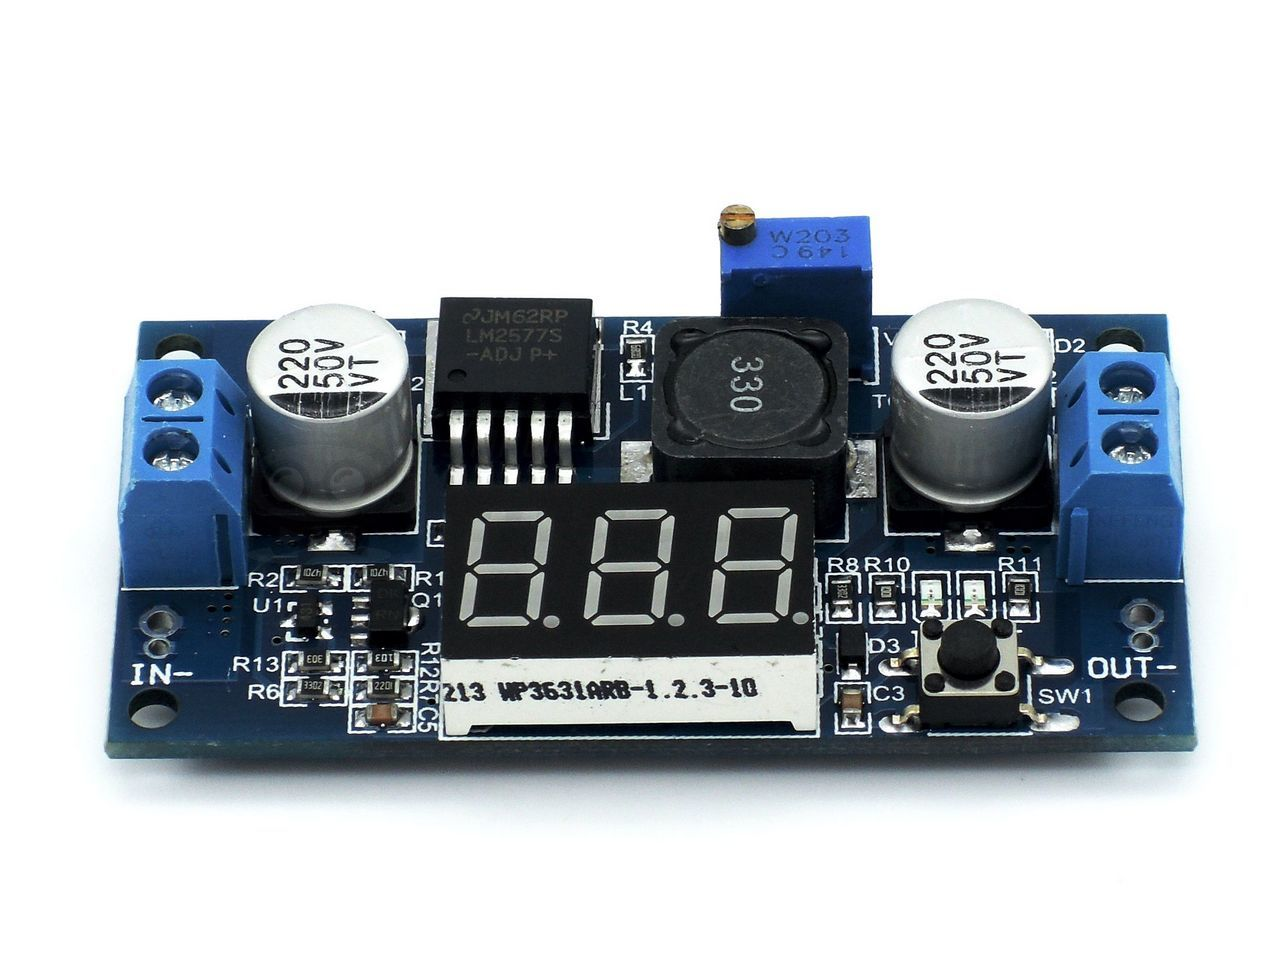
\includegraphics[scale=0.15]{chapter_mechanics_construction/figure5.jpg}
        \caption{Преобразователь на базе \textit{LM2577}}
    \end{subfigure}
     
    \caption{Силовая электроника в составе робота}
    \label{}
\end{figure}

\subsection{Логическая электроника}
В качестве управляющего микрокомпьютера выступает \textit{Raspberry Pi 3B+}. Этого достаточно для совершения множества матричных операций в секунду и для эффективной работы с высокоуровневыми абстракциями в коде.

\begin{figure}[ht]
    \centering
    % левая картинка
    \begin{subfigure}[b]{0.45\textwidth}    
        \centering
        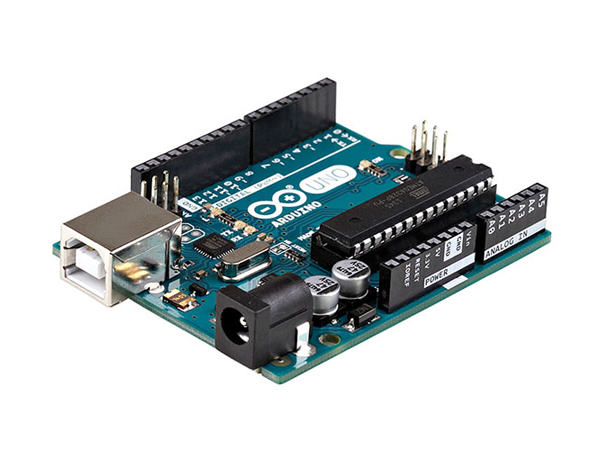
\includegraphics[scale=0.35]{chapter_mechanics_construction/figure3.jpg}
        \caption{\textit{Arduino Uno}}
    \end{subfigure}
    % правая картинка  
    \begin{subfigure}[b]{0.45\textwidth}
        \centering
        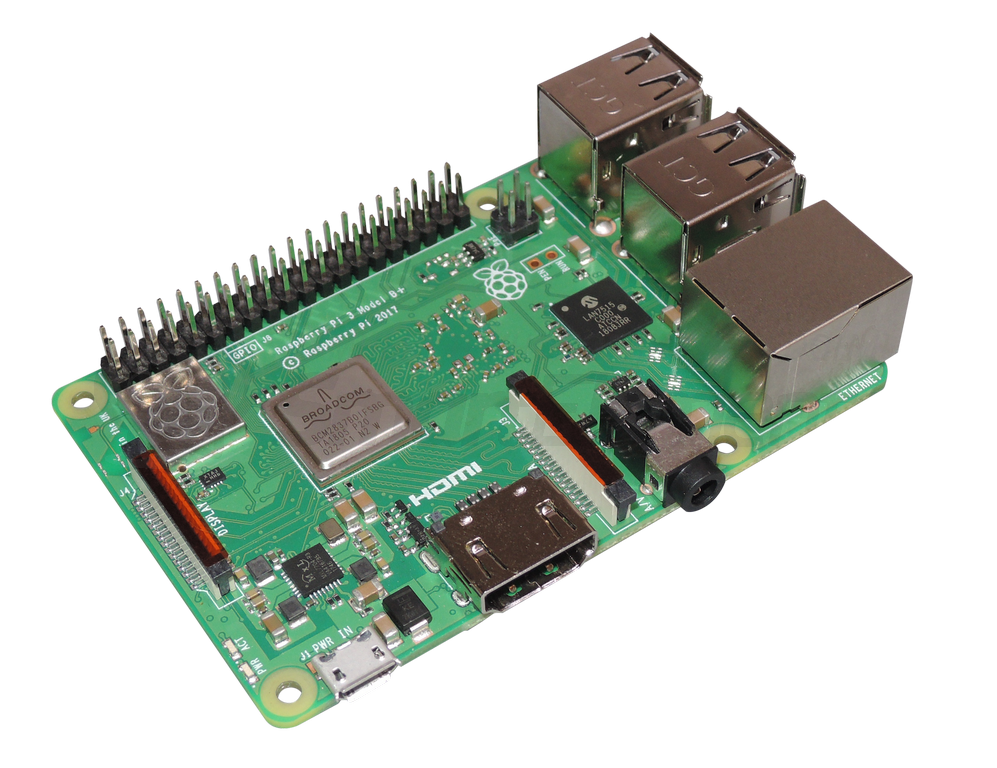
\includegraphics[scale=0.2]{chapter_mechanics_construction/figure3.png}
        \caption{\textit{Raspberry Pi 3B+}}
    \end{subfigure}
     
    \caption{Логическая электроника в составе робота}
    \label{fig:leg_model}
\end{figure}

\textit{Raspberry Pi} выступает исключительно как своеобразный модуль для высокоуровневых вычислений и не работает с <<железом>> напрямую. Вместо этого происходит отправка команд на микроконтроллер в составе платформы \textit{Arduino}. Команды формируются и передаются в цифровом виде на микроконтроллер. Сделано это по двум причинам:
\begin{itemize}
    \item Разграничение логики вычислений состояния робота от процесса управления (подробнее в главе \ref{chap:arch}). % в главе 6 подробнее описано
    \item Электрическая защита дорогостоящего микрокомпьютера от возможных скачков тока в цепи силовой электроники.
\end{itemize}

О протоколе передачи данных и способе формирования команд подробнее написано в пункте \ref{sec:protocol}.

\section{Аккумулятор}
В качестве аккумулятора был использован Литий-полимерный аккумулятор (\textit{Li-Po} аккумулятор). Преимущества аккумуляторов таких типов:
\begin{itemize}
    \item высокая токоотдача;
    \item большая емкость;
    \item быстрая зарядка;
    \item наличие дешевой электроники для контроля разряда таких аккумуляторов;
    \item малый вес и габариты;
\end{itemize}

\begin{figure}[h]
    \centering
    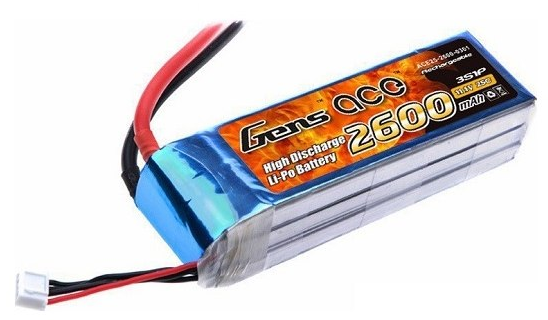
\includegraphics[scale=1]{chapter_mechanics_construction/figure2.png}
    \caption{\textit{Li-Po} аккумулятор на 2600 мА$\cdot$ч}
    \label{}
\end{figure}

С такими большими плюсами существуют и минусы, которые стоит принимать во внимание при эксплуатации такого типа аккумуляторов:
\begin{itemize}
    \item Высокая токоотдача повышает риск получить травму при работе
    \item Высоки шансы на сгорание питающейся от аккумулятора электроники в случае короткого замыкания
    \item Требуются специальные условия хранения, если аккумуляторы долгое время не используются
    \item \textit{Li-Po} аккумуляторы взрывоопасны при неправильной эксплуатации
\end{itemize}


\section{Остальные детали}
Пластиковые детали изготовливались на \textit{3D}-принтере методом \textit{FDM} печати (послойной) из материала \textit{PET-G}, характеристики которого близки к материалу \textit{ABS} \cite{Filament2017}, который широко используется в промышленности, при изготовлении деталей. Преимущества материала для данного робота описаны ниже:
\begin{itemize} % структурировать по-другому
    \item Высокая прочность % пояснить
    \item Термостойкость (выдерживает нагрев до 200 градусов)
    \item Не требователен к условиям печати
    \item Низкая термоусадка (почти не меняет размеры при нагревании/остывании)
    \item Возможность красить и стерилизовать
    \item Не токсичен
\end{itemize}
\begin{figure}[ht]
    \centering
    % левая картинка
    \begin{subfigure}[b]{0.45\textwidth}    
        \centering
        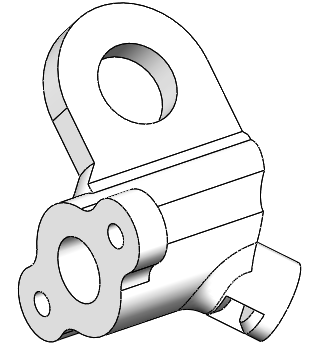
\includegraphics[scale=0.55]{chapter_mechanics_construction/figure21.png}
        \caption{}
    \end{subfigure}
    % правая картинка  
    \begin{subfigure}[b]{0.45\textwidth}
        \centering
        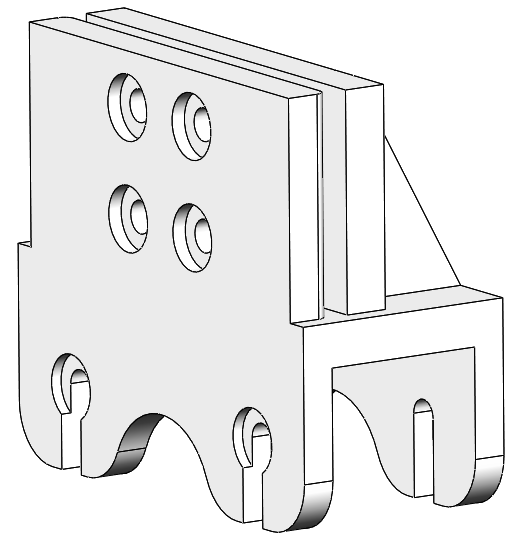
\includegraphics[scale=0.45]{chapter_mechanics_construction/figure22.png}
        \caption{}
    \end{subfigure}
     
    \caption{Примеры деталей, изготовленных на \textit{3D}-принтере}
    \label{}
\end{figure}

Может показаться, что при изготовлени деталей на \textit{3D}-принтере последним можно придавать любую форму, но при \textit{FDM} технологии печати это не так. Технология достаточно дешева и может использоваться в дешевых домашних \textit{3D}-принтерах, поэтому у нее есть свои ограничения на печать <<нависающих>> над печатной областью частей детали. Поэтому при проектировании деталей из пластика нужно исходить из двух принципов. Первый заключается в том чтобы печатать только нестандартные детали, которые невозможно приобрести в розничных магазинах. Второй принцип заключается в том, чтобы использовать в детали как можно меньше материала и скомпоновать ее так, чтобы при печати максимально избежать создания поддержек для нависающих частей. Всё это накладывает свои конструктивные ограничения и требует от конструктора некоторого опыта.

\begin{figure}[h]
    \centering
    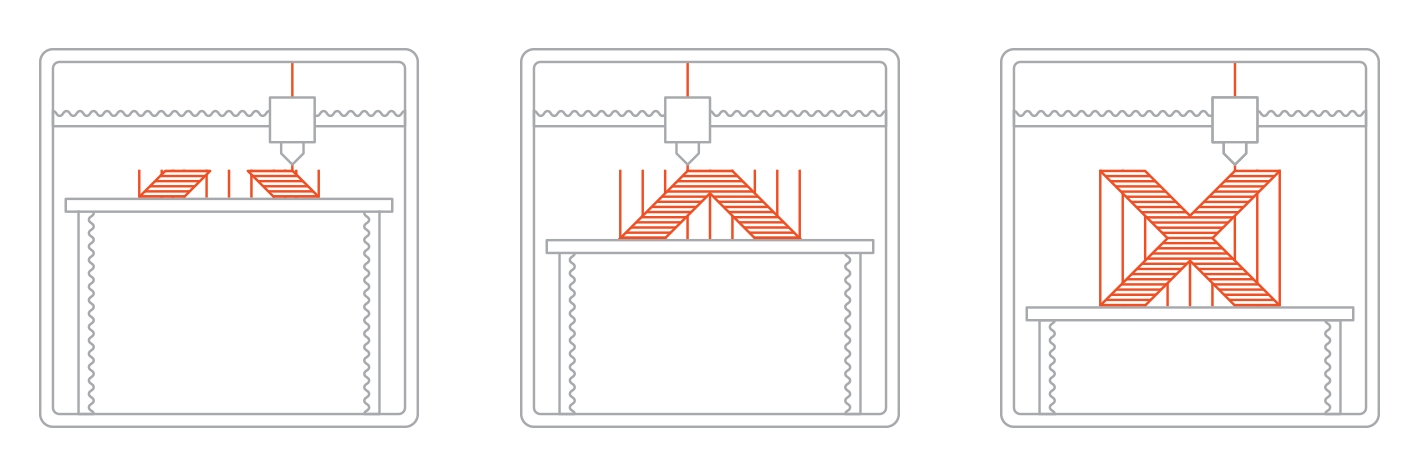
\includegraphics[scale=0.3]{chapter_mechanics_construction/figure1.png}
    \caption{Иллюстрация \textit{3D}-печати по технологии \textit{FDM}}
    \label{}
\end{figure}

Из металла выполнены покупные кронштейны, стержни ног. Стержни -- стандартные полые цилиндрические аллюминиевые профили. Подгонялись под нужную длину при помощи ножовки. Крепление к пластиковым узлам происходило вкручиванием в торцы стержней винтов. Такой способ приводит к хорошему сцеплению деталей.

Для того чтобы избежать разрушения пластиковых деталей в месте вкручивания винта в торец, и из-за невозможности нарезать резьбу в пластиковой детали, были использованы вставки из металлических гаек внутри пластикового материала. В целом, из-за гораздо более низкой прочности пластика по сравнению с металлом, в высоконагруженных местах используется большее количество материала, для снижения напряжений.

В ходе тестирования пластиковых деталей на прочность было выявлено, что 100\% заполнение деталей не делает их более устойчивыми к нагрузкам, делает их хрупкими. В то же время детали, с заполнением от 40\% до 60\% не разрушаются. Теряя свои начальные прочностные характеристики, они деформируются, что положительно сказывается на безопасности находящийся рядом узлов конструкции.

\section*{Результат проектирования}

Сборочный чертеж робота представлен на рисунке \ref{fig:final_drawing}. Фотографии собранного прототипа на рисунках \ref{fig:final_assembly1} и \ref{fig:final_assembly2}.

\begin{figure}[h]
    \centering
    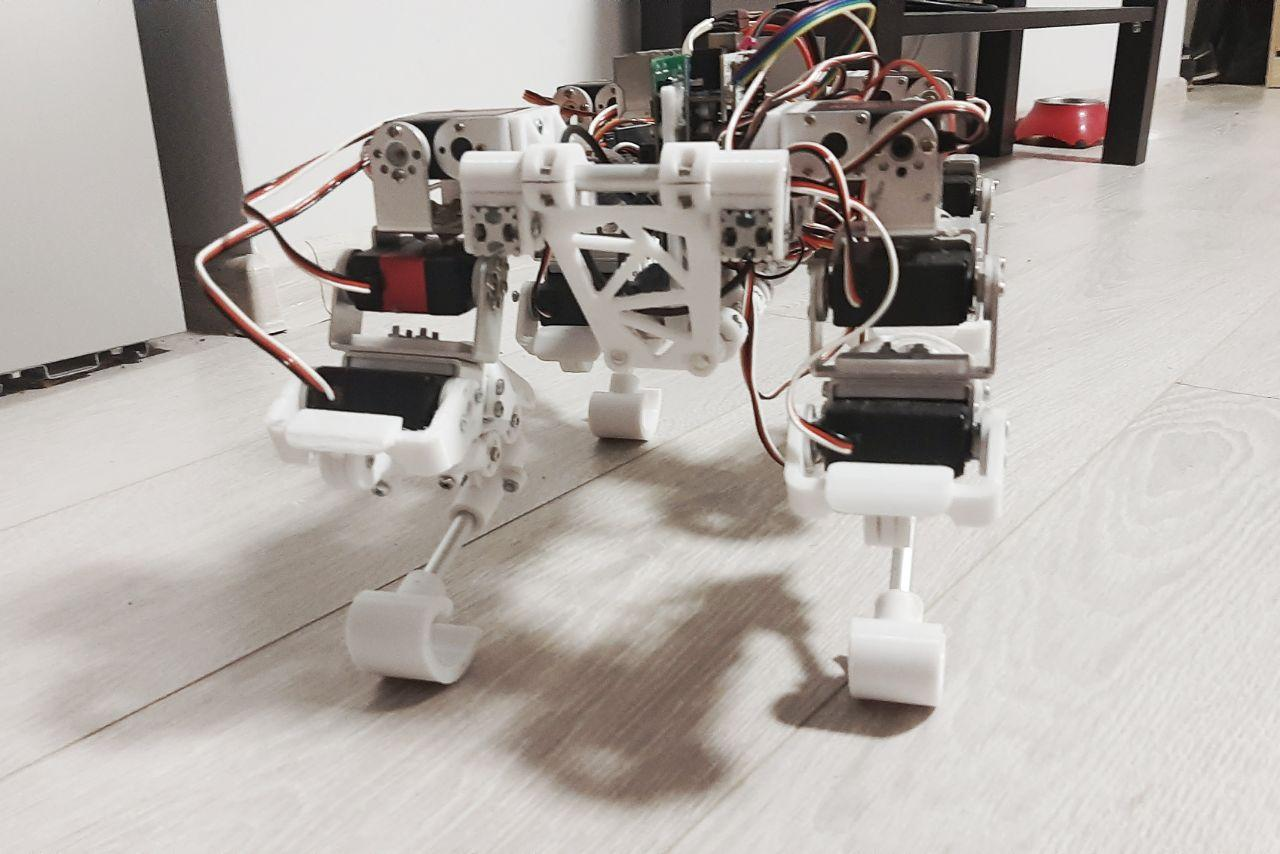
\includegraphics[width=\textwidth]{chapter_mechanics_construction/figure24.jpg}
    \caption{Собранный прототип робота, вид спереди}
    \label{fig:final_assembly1}
\end{figure}

\begin{figure}[h]
    \centering
    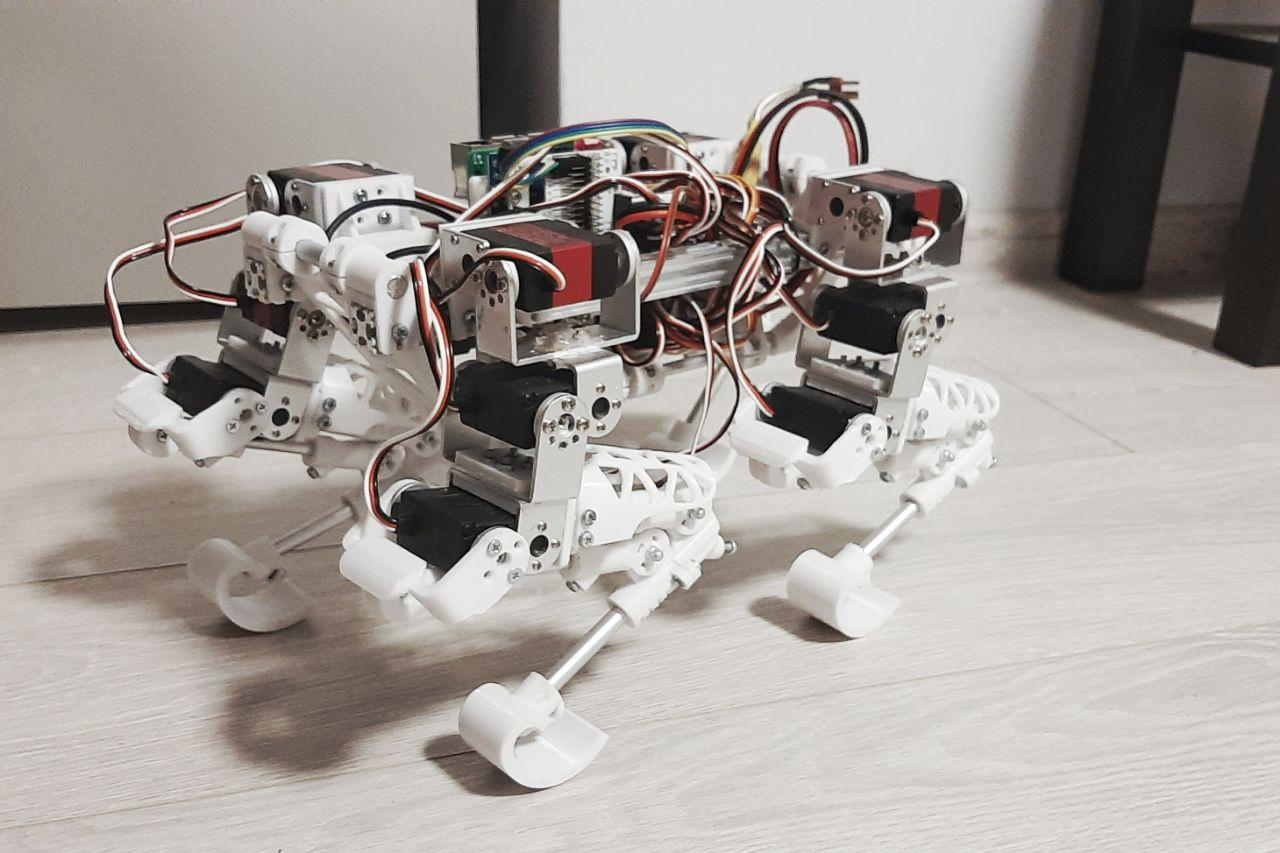
\includegraphics[width=\textwidth]{chapter_mechanics_construction/figure25.jpg}
    \caption{Собранный прототип робота, вид сбоку}
    \label{fig:final_assembly2}
\end{figure}

\begin{figure}[h]
    \centering
    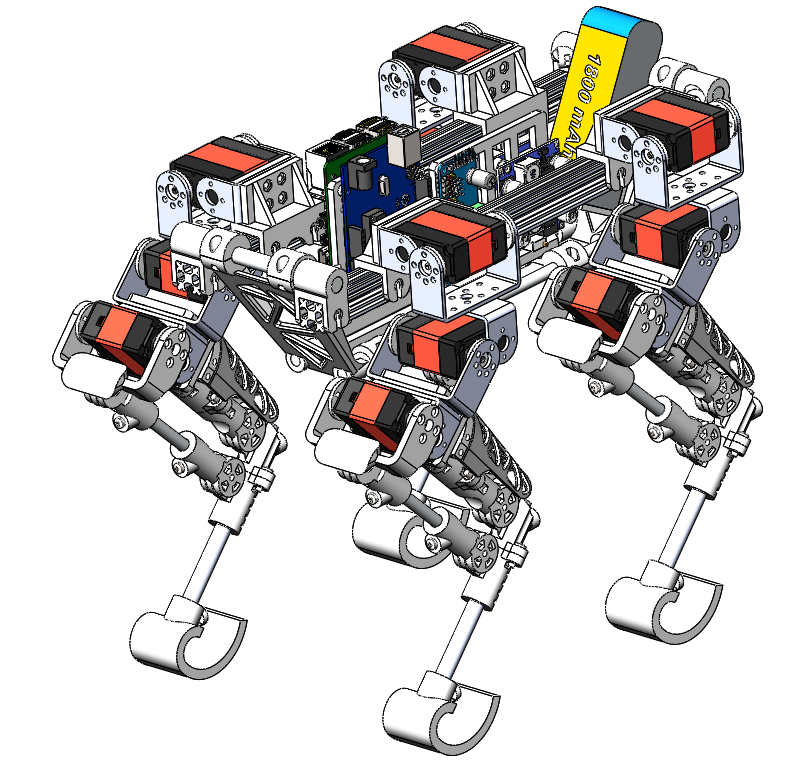
\includegraphics[width=\textwidth]{chapter_mechanics_construction/figure23.png}
    \caption{Чертеж робота в сборке}
    \label{fig:final_drawing}
\end{figure}
